\documentclass[9pt]{beamer}
\usepackage[utf8]{inputenc}
\usepackage{gensymb}
\usepackage{amsmath}
\usepackage{amssymb}
\usepackage{float}
\usepackage{graphicx}
\usepackage{hyperref}
\usepackage{appendix} 
\usepackage[export]{adjustbox}
\usepackage{makecell}
\usepackage{graphicx}
\usepackage{multimedia}
\usepackage{mathtools}
\usepackage[font=scriptsize]{caption}
\usetheme{Boadilla}
%\usepackage{appendix} 
\usepackage{listings}  
\usepackage{mathtools}
\usepackage{multirow}
\usepackage{subcaption}
\usepackage[noabbrev]{cleveref}
%\usepackage{algorithm}
\usepackage{algorithmic}
\usepackage[noend]{algorithm2e}
\usepackage{listings}
\usepackage{pgfplots}
\usepackage{xcolor}
\usepackage[justification=centering]{caption}


\title{Stage M2 MPRI}
\subtitle{Tétraèdres en Diamants : Structure de Données Compacte pour Maillages Tétraédriques}
\author{Gabriel Beauplet supervisé par Luca Castelli Aleardi}
\date{Présentation du 02/09/2019}
\begin{document}
\DeclarePairedDelimiter\bra{\langle}{\rvert}
\DeclarePairedDelimiter\ket{\lvert}{\rangle}
\setlength{\abovecaptionskip}{6pt plus 3pt minus 2pt} % Chosen fairly arbitrarily
\setlength{\belowcaptionskip}{1pt plus 3pt minus 2pt}
\begin{frame}
\titlepage
\begin{figure}

\includegraphics[scale=0.5]{../Rapport/Images/logo_LIX}
\end{figure}
\end{frame}

\begin{frame}
\small
\frametitle{Préliminaires}
%\framesubtitle{Maillages surfaciques et volumiques}
\begin{figure}[H]
\centering
\begin{subfigure}{.5\textwidth}
  \centering
  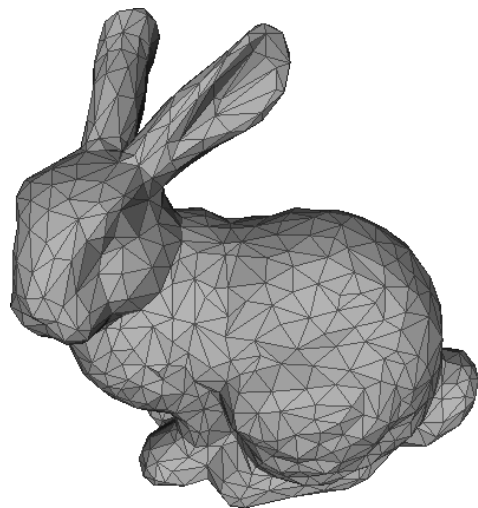
\includegraphics[scale=0.10]{Images/bunny}
  \caption{}
\end{subfigure}%
\begin{subfigure}{.5\textwidth}
  \centering
  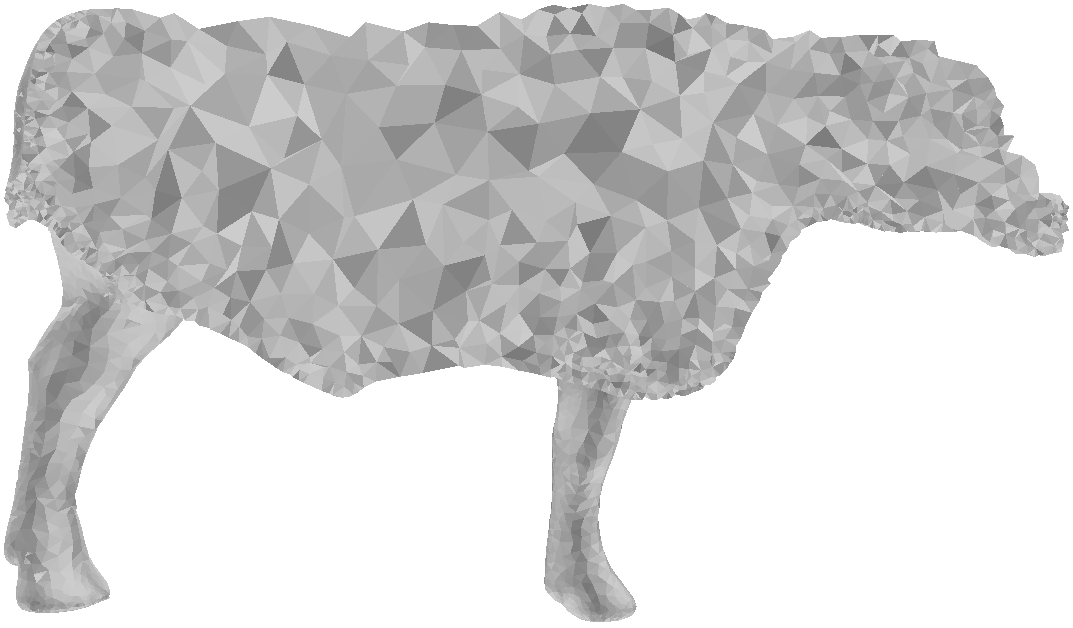
\includegraphics[scale=0.07]{Images/cow_cut}
  \caption{}
\end{subfigure}
\caption{\textbf{Gauche} : Maillage triangulaire (surfacique) contenant 14k sommets, 42k arêtes et 28k faces. \textbf{Droite} : Vue de coupe d'une tétraédrisation (maillage volumique) contenant 30k sommets, 182k arêtes, 143k faces et 134k tétraèdres.}
\end{figure}
\small
\begin{block}{Les maillages}
\begin{itemize}
\item La dimension
\begin{itemize}
\item Les maillages 2D (surfaciques) sont constitués de polygones
\item Les maillages 3D (volumiques) sont constitués de polyèdres
\end{itemize}
\item Ses composantes
\begin{itemize}
\item Géométrie : positions des sommets
\item Connectivité : relations d’adjacence entre les polygones/polyèdres
\end{itemize}
\item Compression et structure de données compacte
\begin{itemize}
\item Compression : réduire la place mémoire du maillage
\item Structure de données compacte : réduire la place mémoire du maillage tout en permettant une utilisation
\end{itemize}
\end{itemize}
\end{block}
\end{frame}

\begin{frame}
\footnotesize
\frametitle{Préliminaires}
%\framesubtitle{Maillages surfaciques et volumiques}
%\begin{figure}[H]
%\centering
%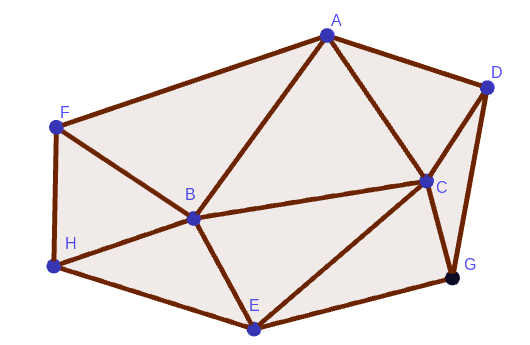
\includegraphics[scale=0.19]{Images/planar_graph}
%\caption{Maillage triangulaire avec bords ($|V|=8$,$|E|=15$,$|F|=9$)}
%\end{figure}

  \begin{columns}[c]
    \begin{column}[c]{.48\textwidth}
 		\begin{block}{Notations}
\begin{itemize}
\item $V$ est l'ensemble des sommets du maillage
\item $E$ est l'ensemble des arêtes du maillage
\item $F$ est l'ensemble des triangles (faces) du maillage
\item $T$ est l'ensemble des tétraèdres du maillage
\end{itemize}
\end{block}
    \end{column}%
    \hfill%
    \begin{column}[c]{.48\textwidth}
    \begin{figure}
    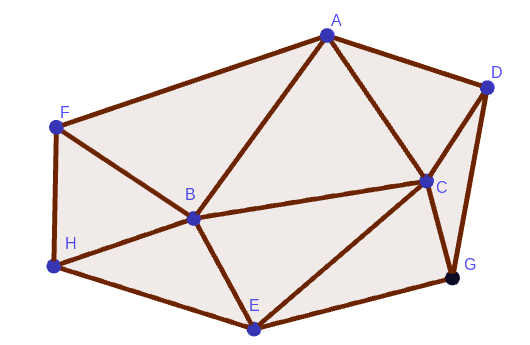
\includegraphics[scale=0.19]{Images/planar_graph}
\caption{Maillage triangulaire avec bords ($|V|=8$,$|E|=15$,$|F|=9$)}
    \end{figure}
    \end{column}%
  \end{columns}


\begin{block}{Définitions}
\begin{itemize}
\item Simplexe : Un simplexe $\sigma^p$ de dimension $p$ est l'enveloppe convexe de $p+1$ points $\{v_0,v_1,...v_p\}$, où $v_i\, \in R^n$ et les vecteurs $v_1-v_0,v_2-v_0...$ sont linéairement indépendants. 
\item Variété  : Espace topologique M connexe séparé localement homéomorphe à un ouvert de $\mathbb{R}^n$. Chaque point de M admet un voisinage homéomorphe à un ouvert de $\mathbb{R}^n$.
\item Complexe Simplicial : Ensemble K de simplexes d'un espace affine tel que toutes les faces de chaque simplexe de K appartiennent aussi à K et si deux simplexes $\sigma$ et $\tau$ de K sont adjacents alors $\sigma \cap \tau \neq \emptyset$
\item Maillage : Complexe simplicial représentant un objet géométrique. Il a la même dimension que l'objet qu'il représente
\item Etoile : Ensemble des k-simplexes adjacents à un sommet
\end{itemize}
\end{block}
\end{frame}

\begin{frame}
\footnotesize
\frametitle{Préliminaires}
%\framesubtitle{Attentes de la structure de données}
\begin{figure}
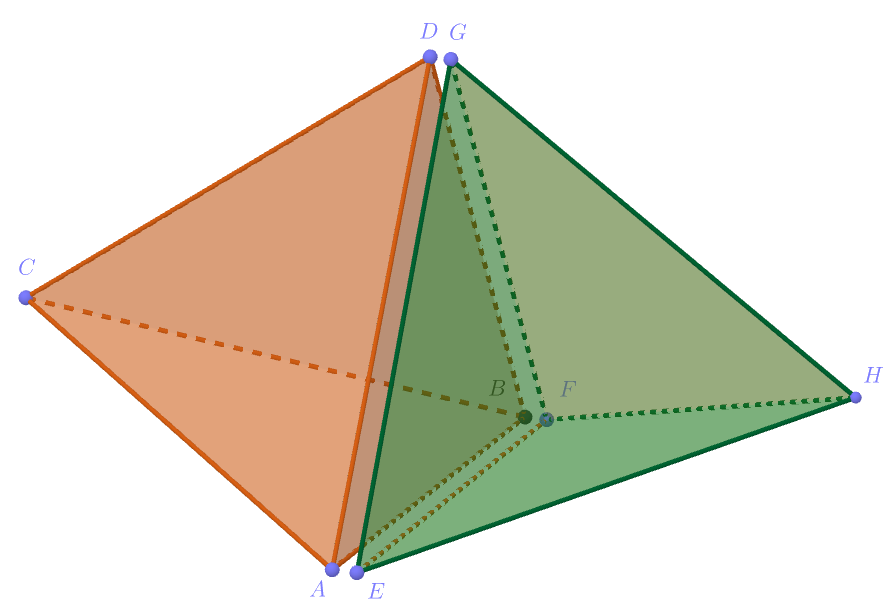
\includegraphics[scale=0.11]{Images/naive}
\caption{Deux tétraèdres partageant une face. Un espace a été ajouté entre les deux tétraèdres pour plus de clarté.}
\end{figure}
\begin{block}{Opérations courantes}
\begin{itemize}
\item \texttt{incident\_face($i,t$)}: renvoie la $i$-ème face du tétraèdre $t$ (pour $i=0..3$)
\item \texttt{incident\_vertex($v$)}: renvoie un des tétraèdres incidents au sommet $v$
\item \texttt{neighbour($i, t$)}: renvoie le tétraèdre qui est le $i$-ème voisin adjacent au tétraèdre $t$
\item \texttt{get\_vertex\_index($v,t$)}: renvoie un entier $i\in\{0 \ldots 3 \}$, l'indice du sommet $v$ dans le tétraèdre $t$
\end{itemize}
\end{block}

\begin{block}{Une implémentation naïve}
\begin{itemize}
\item $4$ références par tétraèdre donnant l'accès aux tétraèdres voisins
\item $4$ références par tétraèdre donnant l'accès aux sommets incidents
\item $1$ référence par sommet donnant l'accès à l'un de ses tétraèdres incidents
\end{itemize}
$\Rightarrow$ \textbf{8 références par tétraèdre (rpt) et 1 référence par sommet}
\end{block}
\end{frame}

%\begin{frame}
%\frametitle{Préliminaires}
%\framesubtitle{Géométrie et connectivité}
%%  \begin{columns}[c]
%%    \begin{column}[c]{.48\textwidth}
%% 		\begin{block}{\rlap{Portrait of Simonetta Vespucci}}
%% 		\end{block}
%%    \end{column}%
%%    \hfill%
%%    \begin{column}[c]{.48\textwidth}
%%  	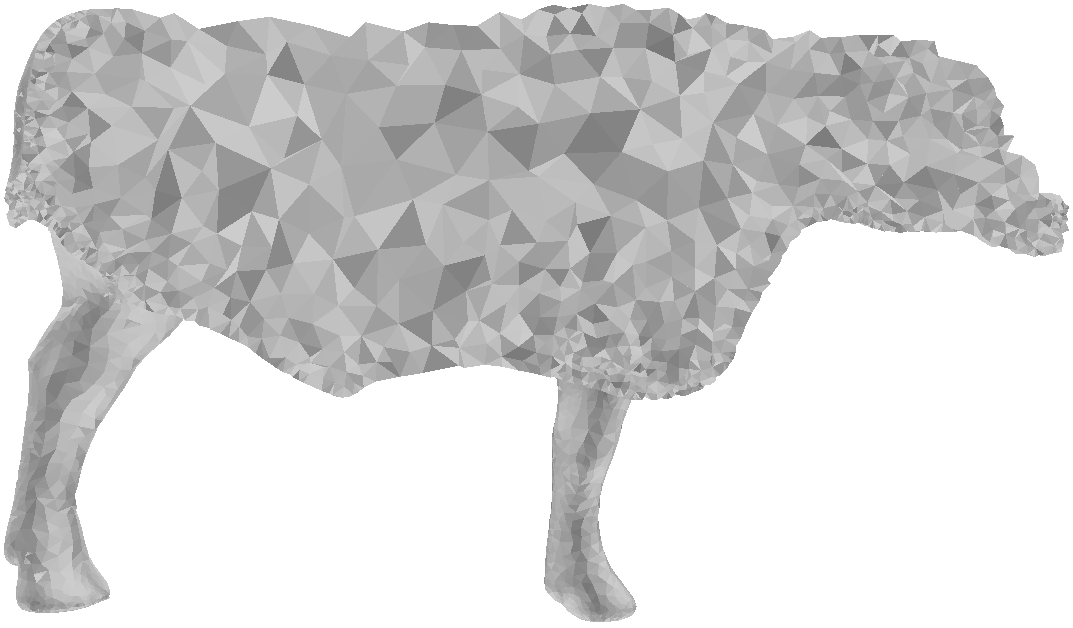
\includegraphics[scale=0.14]{Images/cow_cut}
%%    \end{column}%
%%  \end{columns}
%\small


%\begin{block}{Cas surfacique (triangulaire)}
%\begin{itemize}
%\item Géométrie : 1 référence par sommet
%\item Connectivité :
%\begin{itemize}
%\item 1 référence par sommet vers un triangle adjacent
%\item 3 références par triangle vers ses sommets
%\item 3 références par triangle vers ses triangles voisins
%\end{itemize}
%\end{itemize}
%\end{block}
%
%\begin{block}{Cas volumique (tétraédrique)} 
%\begin{itemize}
%\item Géométrie : 1 référence par sommet
%\item Connectivité :
%\begin{itemize}
%\item 1 référence par sommet vers un tétraèdre adjacent
%\item 4 références par tétraèdre vers ses sommets
%\item 4 références par tétraèdre vers ses tétraèdres voisins
%\end{itemize}
%\end{itemize}
%\end{block}
%\small
%\textbf{Nous nous intéressons dans la suite de ce rapport aux maillages volumiques tétraédriques
%}
%\end{frame}



\begin{frame}
\small
\frametitle{Etat de l'Art}
\framesubtitle{Structures de données surfaciques et volumiques}
\begin{table}[H]
\centering
\footnotesize
\scalebox{0.8}{
\begin{tabular}{|c | c | c | c | c|}
\hline
Structure de données & Taille mémoire & Temps de navigation & Accès au sommet & Dynamique\\
\hline
Basées sur les arêtes & \multirow{2}{*}{18n+n} & \multirow{2}{*}{O(1)} & \multirow{2}{*}{O(1)} &\multirow{2}{*}{oui}\\
(Half-edge, Quad-edge, Winged-edge)&&&&\\
Basées sur les triangles & 13n & O(1) & O(1) & oui\\		
Corner table & 13n & O(1) & O(1) & oui\\
\hline
2D catalog (Aleardi, Devillers, Mebarki)& 7.67n & O(1) & O(1) & oui\\
\hline
Star vertices (Kallmann, Thalmann) & 7n & O(d) & O(1) & non\\		
SOT (Gurung,Rossignac)& 6n & O(1) & O(d) & non\\
SQUAD (Gurung, Laney, Lindstrom, Rossignac)& $(4+\epsilon)$n & O(1) & O(d) & non\\
%LR & $(2+\delta)$n & O(1) & O(d) & non\\
\hline  
\end{tabular}
}
\caption{Taille mémoire et performances des structures de données pour maillages surfaciques. n représente le nombe de sommets.}
\end{table}

\begin{table}[th]
\centering
\footnotesize
\scalebox{0.75}{
\begin{tabular}{|c | c | c | c | c|}
\hline
Structure de données & Taille mémoire moyenne & Temps de navigation & Accès au sommet & Dynamique\\
\hline
VOT & 8t+n & O(1) & O(1) & oui \\
Compact Half Face (Lage, Lewiner, Lopes, Velho) & 8t+n & O(1) & O(1) & oui\\
Bande de triangles (Weiler, Mallón, Kraus, Ertl) & 5.1t & O(1) & O(1) & non \\
SOT (Gurung, Rossignac) & 4t & O(1) & O(d)  & non\\
\textbf{Tétraèdres en diamants} & \textbf{ 2.4t } & \textbf{O(1)} & \textbf{O(d)} & \textbf{non} \\
\hline  
\end{tabular}
}
\caption{Taille mémoire et performances des structures de données pour maillages volumiques. t représente le nombre de tétraèdres et n le nombre de sommets.}
\end{table}
\end{frame}

\begin{frame}
\small
\frametitle{Notre Structure : Tétraèdres en Diamants}
\framesubtitle{Principe général}
\small
\begin{block}{Notre but}
\begin{itemize}
\item Construire une structure de données compacte pour maillages tétraédriques
\item Construction rapide de la structure
\item Navigation en temps constant
\item Calcul de l'hypersphère d'un sommet
\end{itemize}
\end{block}
\begin{block}{Procédure}
\begin{itemize}
\item Etape 1 : Groupement des tétraèdres en diamants (\textit{SQUAD})
\item Etape 2 : Ancrage des sommets avec des diamants/tétraèdres isolés. Le $i$-ème sommet est ancré au $i$-ème diamant/tétraèdre isolé (\textit{SOT})
\item Etape 3 : Encodage des références. Passage d'un tétraèdre à l'autre en utilisant les faces (\textit{Half-Face})
\end{itemize}
\end{block}
\end{frame}

\begin{frame}
\small
\frametitle{Notre Structure : Tétraèdres en Diamants}
\framesubtitle{Etape 1 : Groupement des tétraèdres en diamants}
\begin{figure}[H]
\centering
\begin{subfigure}{.24\textwidth}
  \centering
  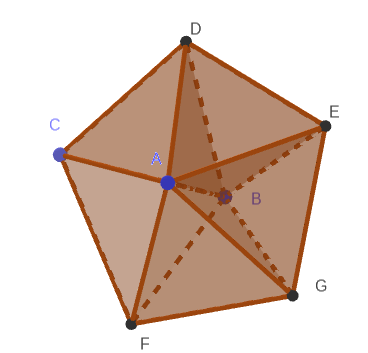
\includegraphics[scale=0.21]{Images/full_diamond}
  \caption{}
\end{subfigure}%
\begin{subfigure}{.24\textwidth}
  \centering
  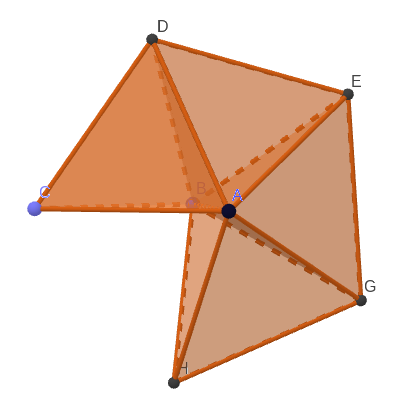
\includegraphics[scale=0.17]{Images/not_full_diamond}
  \caption{}
\end{subfigure}
\begin{subfigure}{.24\textwidth}
  \centering
  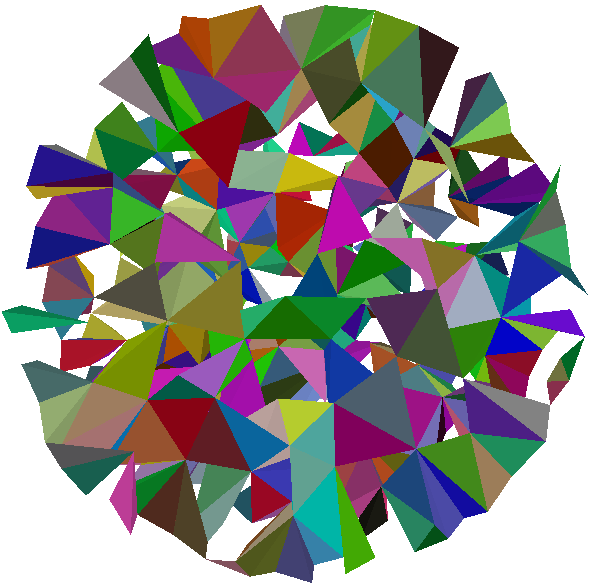
\includegraphics[scale=0.12]{Images/isolated_tetra}
  \caption{}
\end{subfigure}
\begin{subfigure}{.24\textwidth}
  \centering
  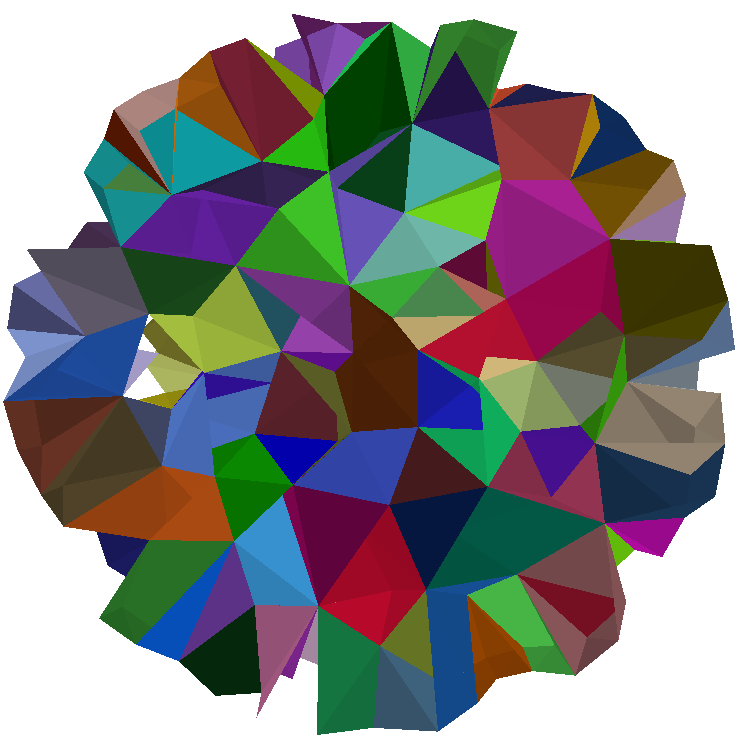
\includegraphics[scale=0.095]{Images/diamond}
  \caption{}
\end{subfigure}
\caption{\textbf{(a)} : Diamant contenant 5 tétraèdres et dont l'arête centrale commune est AB. \textbf{(b)} : Exemple n'étant pas un diamant car les tétraèdres ne sont pas cycliques. \textbf{(c)} : Vue de coupe des tétraèdres isolés après exécution du parcours en largeur pour créer les diamants. Chaque couleur représente un tétraèdre isolé. \textbf{(d)} : Vue de coupe des diamants après exécution du parcours en largeur pour créer les diamants. Chaque couleur représente un diamant.}
\end{figure}
\begin{block}{Etape 1}
\begin{itemize}
\item Problème : Grouper les tétraèdres en diamants
\item Motif : Omission des références entre les tétraèdres du même diamant
\begin{itemize}
\item Deux voisins dans un diamant ne se référenceront pas mutuellement. Chaque tétraèdre dans le diamant n'aura donc que deux références vers ses voisins extérieurs au diamant
\end{itemize}
\item Solution : Parcours en profondeur du maillage
\item Résultat : Une partie des tétraèdres est groupé en diamants. Les autres tétraèdres sont dits isolés
\end{itemize}
\end{block}
\end{frame}

\begin{frame}
\small
\frametitle{Notre Structure : Tétraèdres en Diamants}
\framesubtitle{Etape 2 : Ancrage des sommets}
\begin{figure}[H]
\centering
\begin{subfigure}{.32\textwidth}
  \centering
  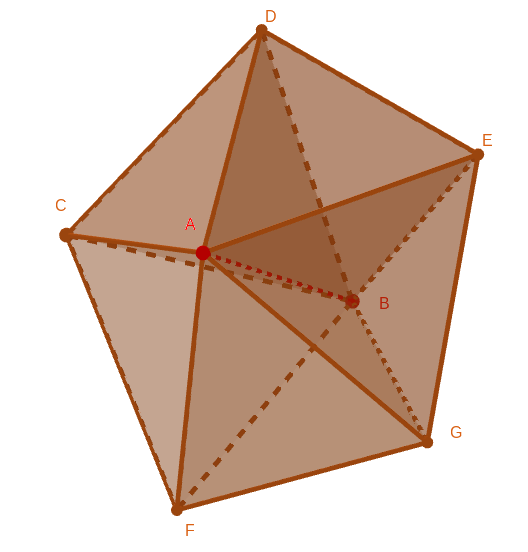
\includegraphics[scale=0.12]{Images/central_edge_AB}
  \caption{}
  \label{fig:central_edge_AB}
\end{subfigure}%
\begin{subfigure}{.32\textwidth}
  \centering
  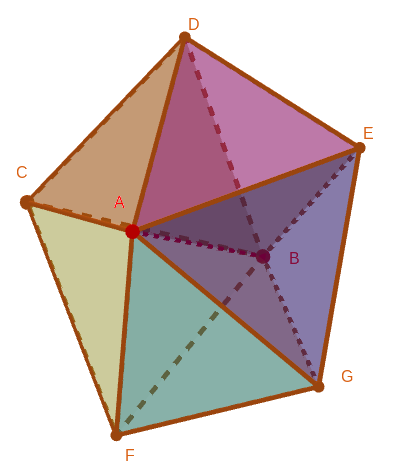
\includegraphics[scale=0.16]{Images/explosion_diamond}
  \caption{}
  \label{fig:explosion_diamond}
\end{subfigure}
\begin{subfigure}{.32\textwidth}
  \centering
  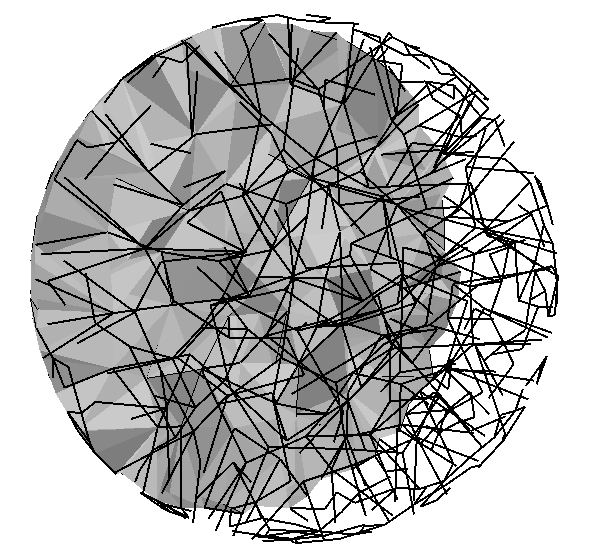
\includegraphics[scale=0.12]{Images/central_edges}
  \caption{}
\end{subfigure}
\caption{\textbf{Gauche} : Diamant contenant 5 tétraèdres dont l'arête centrale est le segment AB et ancré au sommet A. \textbf{Milieu} : 5 tétraèdres isolés (chaque couleur est un tétraèdre différent). \textbf{Droite} : Vue de coupe d'une tétraédrisation d'une boule avec affichage des arêtes centrales de tous les diamants}
\end{figure}

\begin{block}{Etape 2}
\begin{itemize}
\item Problème : Ancrer chaque sommet à un tétraèdre/diamant
\item Motif : Omission des références des sommets vers l'un de leurs tétraèdres incidents
\item Solution : Algorithme glouton privilégiant les sommets de faible degré
\item Résultat : Chaque sommet est ancré à un diamant/tétraèdre isolé. On réordonne les diamants/tétraèdres isolés tel que le $i$-ème sommet soit ancré au $i$-ème diamant/tétraèdre isolé
\end{itemize}
\end{block}
\end{frame}

\begin{frame}
\small
\frametitle{Notre Structure : Tétraèdres en Diamants}
\framesubtitle{Organisation générale}

\begin{figure}[H]
\centering
\begin{subfigure}{.5\textwidth}
  \centering
  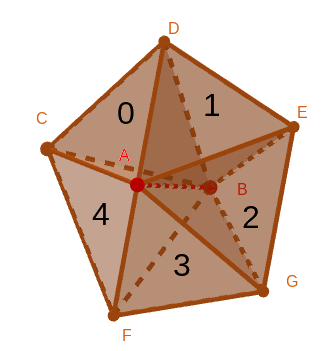
\includegraphics[scale=0.19]{Images/tetra_ordonnee}
  \caption{}
\end{subfigure}%
\begin{subfigure}{.5\textwidth}
  \centering
  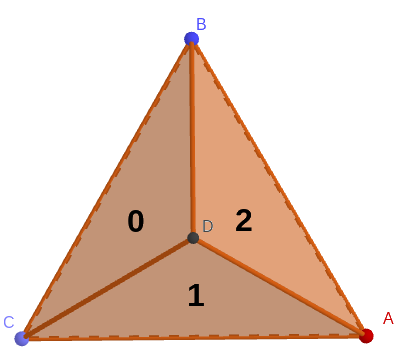
\includegraphics[scale=0.16]{Images/tetra_number_face}
  \caption{}
\end{subfigure}
\caption{\textbf{Gauche} : Diamant contenant 5 tétraèdres ordonnés, dont l'arête centrale est AB et ancré au sommet A. L'ordre des tétraèdres est indiqué en noir. \textbf{Droite} : Tétraèdre isolé ancré au sommet A.}
\end{figure}
\begin{block}{Règles pour l'ordonnancement}
\begin{itemize}
\item Diamant
\begin{itemize}
\item L'ordre de deux tétraèdres partageant une face doit être consécutif modulo la taille du diamant
\item Les faces extérieures du $i$-ème tétraèdre seront les faces $2i$ et $2i+1$
\item On ordonne d'abord les sommets situés entre deux faces, puis les deux sommets communs à toutes les faces
\end{itemize}
\item Tétraèdre isolé
\begin{itemize}
\item S'il est ancré à un sommet, alors la première face doit être la face opposée à l'ancre
\item Les sommets sont ordonnés tel que le $i$-ème sommet est opposé à la $i$-ème face
\end{itemize}
\end{itemize}
\end{block}
\end{frame}

\begin{frame}
\frametitle{Notre Structure : Tétraèdres en Diamants}
\framesubtitle{Etape 3 : Encodage des références}
\small
\begin{block}{La situation}
\begin{itemize}
\item Les tétraèdres sont regroupés en diamants ou isolés
\item Chaque sommet est associé avec un diamant ou un tétraèdre isolé
\end{itemize}
\end{block}

\begin{block}{Notations}
\begin{itemize}
\item $D$ l'ensemble des diamants
\item $T_D$ l'ensemble des tétraèdres appartenant à des diamants
\item $T_i$ l'ensemble des tétraèdres isolés
\item $F_e$ l'ensemble des faces des tétraèdres isolés et des faces extérieures des diamants où $|F_e|=2\cdot |T_D|+4\cdot |T_i|$\\
\end{itemize}
\end{block}

\begin{block}{Comment définir les références ?}
\begin{itemize}
\item On numérote toutes les faces extérieures $f \in F_e$ de notre maillage
\item Une référence est juste un numéro de face
\item Chaque $f \in F_e$ possède une référence vers une autre face
\end{itemize}
\end{block}

\end{frame}

\begin{frame}
\small
\frametitle{Notre Structure : Tétraèdres en Diamants}
\framesubtitle{Identification des sommets dans des tétraèdres/diamants opposés}
\begin{figure}[H]
\centering
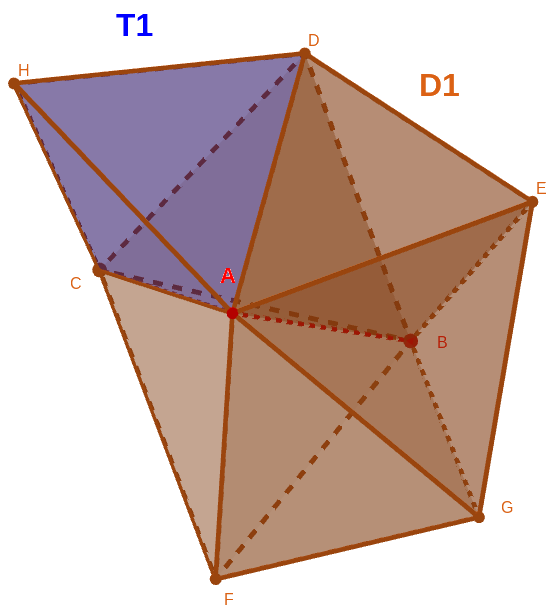
\includegraphics[scale=0.21]{Images/permut1}
\caption{Tétraèdre isolé \textcolor{blue}{\textbf{T1}} partageant la face ACD avec un diamant \textcolor{brown}{\textbf{D1}} ancré au sommet \textcolor{red}{\textbf{A}}.}
\end{figure}
\begin{block}{Notre situation}
\begin{itemize}
\item Le sommet \textcolor{red}{\textbf{A}} est ancré au tétraèdre \textcolor{brown}{\textbf{D1}}
\item Nous sommes sur la face ACD de \textcolor{brown}{\textbf{D1}}
\item\textbf{Comment savoir où se trouve le sommet \textcolor{red}{\textbf{A}} dans \textcolor{blue}{\textbf{T1}} ?}
\end{itemize}
\end{block}
\end{frame}

\begin{frame}
\frametitle{Notre Structure : Tétraèdres en Diamants}
\framesubtitle{Identification des sommets dans des tétraèdres/diamants opposés}
\begin{figure}[H]
\centering
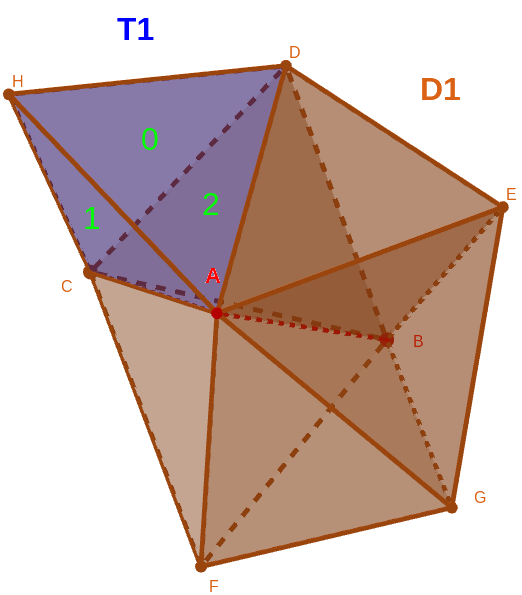
\includegraphics[scale=0.14]{Images/permut2}
\caption{Un diamant partage la face ACD avec un tétraèdre isolé. }
\end{figure}
\scriptsize
\begin{block}{Organisation des sommets et des faces}
\begin{itemize}
\item L'ordre des sommets de \textcolor{blue}{\textbf{T1}} est : A,D,C,H \textbf{$\Rightarrow$} l'ordre des faces de \textcolor{blue}{\textbf{T1}} est DCH,ACH,ADH,ADC
\item L'ordre des faces de \textcolor{brown}{\textbf{D1}} est : ACD,BCD,ADE,BDE,AEG,BEG,EFG,BFG,AFC,BFC \textbf{$\Rightarrow$} l'ordre des sommets de \textcolor{brown}{\textbf{D1}} est C,D,E,G,F,A,B
\end{itemize}
\end{block}
\begin{block}{Calculer la permutation}
\begin{itemize}
\item On identifie la face (et ses 3 sommets) dont on souhaite savoir la permutation
\begin{itemize}
\scriptsize
\item La face ACD nous intéresse
\end{itemize}
\item On compare l'ordre des sommets dans les deux entités
\begin{itemize}
\scriptsize
\item Dans \textcolor{blue}{\textbf{T1}}, nous avons A,D,C et C,D,A dans \textcolor{brown}{\textbf{D1}} 
\end{itemize}
\end{itemize}
\textbf{La permutation des sommets pour la face ACD est donc $\tau$=(2,1,0)}
\end{block}
\end{frame}


\begin{frame}
\small
\frametitle{Notre Structure : Tétraèdres en Diamants}
\framesubtitle{Description}

\begin{figure}[H]
\begin{center}
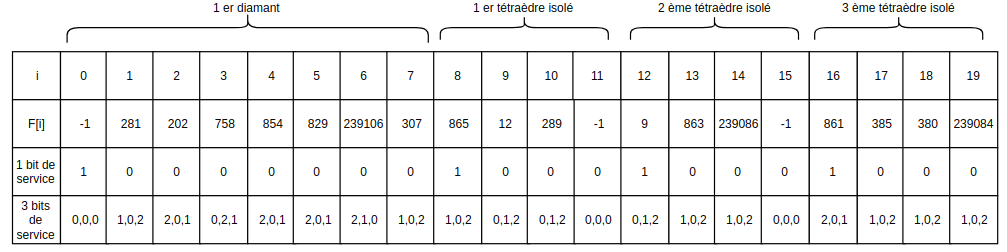
\includegraphics[scale=0.275]{Images/structure}
\caption{Dans cet exemple, la face 0 est sur le bord et la face 1 est opposée à la face 281. La permutation de la face 1 du premier diamant (1,0,2) indique que le premier et second sommet de cette face sont inversés dans la face opposée.}
\label{fig:structure}
\end{center}
\end{figure}




%\begin{block}{Contenu}
%\small
%\begin{itemize}
%\item Un tableau A de taille $|F_e|$
%\item Un bit de service par face afin de savoir si une face est la première d'un diamant ou d'un tétraèdre isolé
%\item 3 bits de service par face afin de représenter la permutation des sommets entre deux faces
%\end{itemize}
%\end{block}

\end{frame}

%
%\begin{frame}
%\frametitle{Notre Structure : Tétraèdres en Diamants}
%\framesubtitle{Exemple}
%\begin{figure}[H]
%\begin{center}
%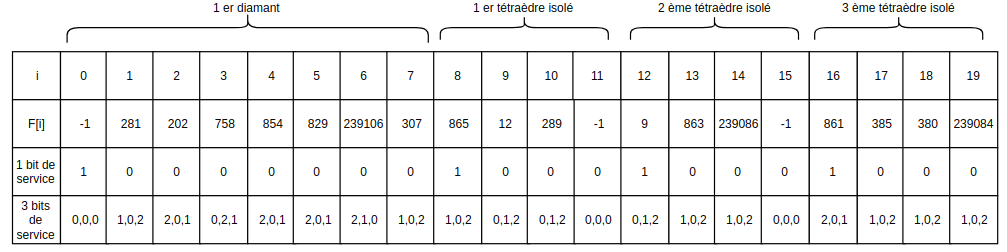
\includegraphics[scale=0.27]{Images/structure}
%\caption{Dans cet exemple, la face 0 est sur le bord et la face 1 est opposée à la face 281. La permutation de la face 1 du premier diamant (1,0,2) indique que le premier et second sommet de cette face sont inversés dans la face opposée.}
%\label{fig:structure}
%\end{center}
%\end{figure}
%\end{frame}


\begin{frame}
\frametitle{Résultats}
\framesubtitle{Appariement des diamants et ancrage des sommets}
\begin{block}{Compter le nombre de références par tétraèdre (rpt)}
\begin{equation}
\text{RPT} = \frac{2\cdot T_D+4\cdot T_i}{|T|}
\end{equation}
\end{block}
\end{frame}

\begin{frame}
\frametitle{Résultats}
\framesubtitle{Les requêtes}
\begin{figure}[H]
\centering
\resizebox{0.8\textwidth} {!}{
\pgfplotsset{width=12cm,height=7cm}
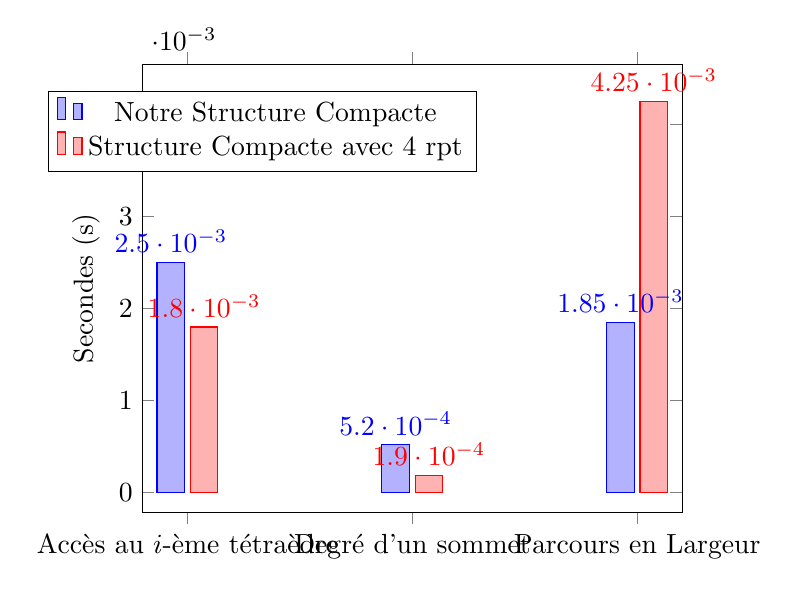
\begin{tikzpicture}
\begin{axis}[
    ybar,
    enlargelimits=0.1,
%    legend style={anchor=east},
    legend style={at={(0.62,0.94)}},
%    anchor=north,legend columns=-1,cells={align=left}},
    ylabel={Secondes (s)},
%    xlabel={Nombre de tétraèdres par arête},
    symbolic x coords={Accès au $i$-ème tétraèdre,Degré d'un sommet,Parcours en Largeur},
    xtick=data,
    nodes near coords,
    nodes near coords align={vertical},
    ]
\addplot coordinates {(Accès au $i$-ème tétraèdre,2.5e-3)(Degré d'un sommet,5.2e-4)(Parcours en Largeur,1.85e-3)};
\addplot coordinates {(Accès au $i$-ème tétraèdre,1.8e-3)(Degré d'un sommet,1.9e-4)(Parcours en Largeur,4.25e-3)};
%\addplot coordinates {(Degré d'un sommet,1e-3)(Parcours en Largeur,2.92e-3)};
%\addplot coordinates {(3.9,2.36)(4.29,2.38)(4.43,2.34)(4.93,2.29)(5.08,)(5.10,)(5.11,) };
\legend{Notre Structure Compacte,Structure Compacte avec 4 rpt,Structure avec Pointeurs}
\end{axis}
\end{tikzpicture}
}
\caption{Comparaison des temps moyens (s) requis pour répondre aux requêtes et effectuer la navigation dans le maillage. Notre structure de données compacte (en bleue) est comparée à une  structure de données compacte utilisant 4 rpt (i.e SOT). Le temps pour le parcours en largeur est normalisé pour 100K tétraèdres.}
\label{fig:temps_moyen}
\end{figure}
\end{frame}

\begin{frame}
\frametitle{Résultats}
\framesubtitle{Taille mémoire}
\begin{figure}[H]
\centering
\resizebox{0.8\textwidth} {!}{
\pgfplotsset{width=13cm,height=7cm}
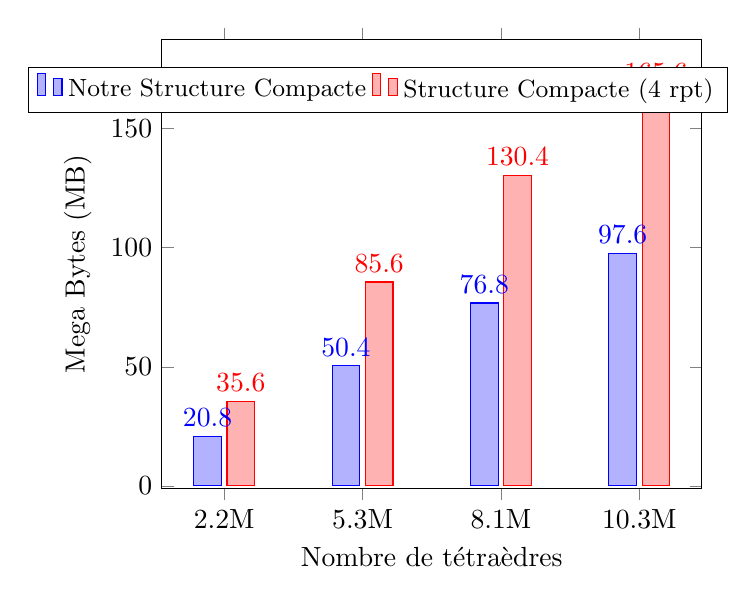
\begin{tikzpicture}
\begin{axis}[
    ybar,
%    ymode = log,
    enlargelimits=0.15,
    legend style={at={(0.4,0.94)},
      anchor=north,legend columns=-1,font=\fontsize{9}{9}\selectfont},
    ylabel={Mega Bytes (MB)},
    xlabel={Nombre de tétraèdres},
    symbolic x coords={2.2M,5.3M,8.1M,10.3M},
    xtick=data,
    nodes near coords,
    nodes near coords align={vertical},
    ]
%\addplot coordinates {(3k,9234)(83k,199262)(125k,307500)(156k,384156)(2.2M,5291508)(8.1M,19212158)(10.3M,24407986)};
%\addplot coordinates {(3k,14332)(83k,333648)(125k,500508)(156k,624540)(2.2M,8.97e6)(8.1M,3.26e7)(10.3M,4.14e7)};
\addplot coordinates {(2.2M,20.8)(5.3M,50.4)(8.1M,76.8)(10.3M,97.6)};
\addplot coordinates {(2.2M,35.6)(5.3M,85.6)(8.1M,130.4)(10.3M,165.6)};
\legend{Notre Structure Compacte,Structure Compacte (4 rpt)}
\end{axis}
\end{tikzpicture}
}
\caption{Comparaison de la taille mémoire (en Mega Bytes) de notre structure de données compacte (en bleue) et de la même structure de données sans regroupement des tétraèdres en diamants (i.e SOT)}
\label{fig:taille_memoire}
\end{figure}
\end{frame}

\begin{frame}
\frametitle{Conclusion}
\begin{figure}[H]
\centering
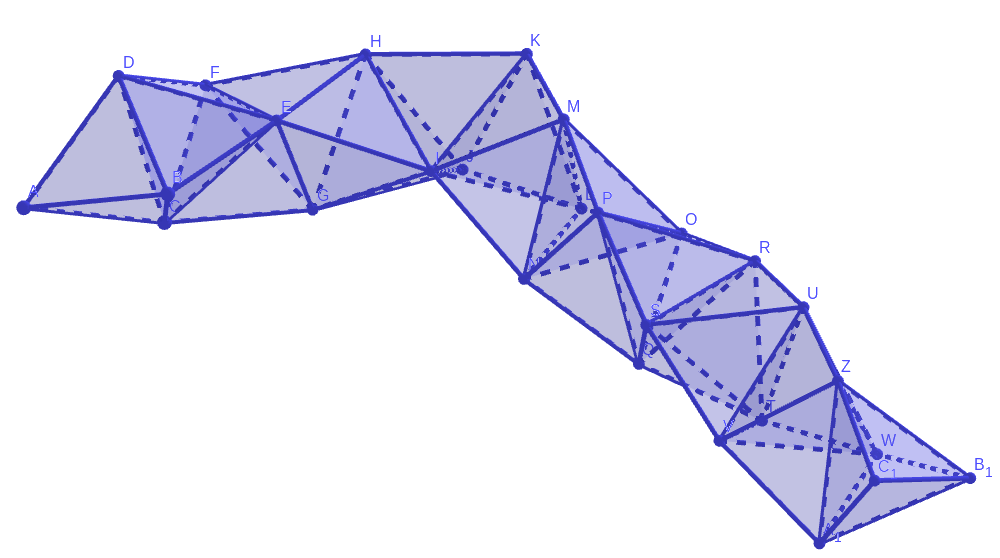
\includegraphics[scale=0.1]{Images/serpentin}
\caption{Serpentin de tétraèdres. Aucun diamant n'est réalisable}
\end{figure}
\begin{block}{Avantages et inconvénients}
\begin{itemize}
\color{blue}
\item 40\% plus économe en références que l'état de l'art (i.e SOT)
\item Navigation en O(1) et calcul de l'hypersphère d'un sommet en O(d)
\item Facilement implémentable
\item Sauvegarde plus concise d'un maillage tétraédrique
\color{red}
\item Notre structure peut utiliser jusqu'à 4 RPT
\item La lecture des tétraèdres afin de créer les diamants est un réel frein
\end{itemize}
\color{blue}
\end{block}
\begin{block}{Travail futur}
\begin{itemize}
\item Rendre la structure dynamique
\item Etendre la structure de données à des maillages non tétraédriques
\end{itemize}
\end{block}
\end{frame}




\end{document}